\documentclass[lettersize,journal]{IEEEtran}
\usepackage{amsmath,amsfonts}
\usepackage{algorithmic}
\usepackage{array}
\usepackage[caption=false,font=normalsize,labelfont=sf,textfont=sf]{subfig}
\usepackage{textcomp}
\usepackage{stfloats}
\usepackage{url}
\usepackage{verbatim}
\usepackage{graphicx}
\usepackage{amsfonts}
\usepackage{amsmath}
\usepackage{amssymb}
\usepackage{amsthm}
\usepackage{pdfpages}
\usepackage{amssymb}
\usepackage{listings}
\usepackage{proof}
\usepackage{xcolor}
\usepackage{titlesec}
\usepackage{rotating}
\usepackage{float}
\usepackage{tikz}
\hyphenation{op-tical net-works semi-conduc-tor IEEE-Xplore}
\def\BibTeX{{\rm B\kern-.05em{\sc i\kern-.025em b}\kern-.08em
    T\kern-.1667em\lower.7ex\hbox{E}\kern-.125emX}}
\usepackage{balance}

\definecolor{OliveGreen}{rgb}{0,0.6,0}
\lstset{
  language=C,
  frame=tb,
  aboveskip=3mm,
  basicstyle=\footnotesize\ttfamily,
  numbers=left,
  stepnumber=1,
  numbersep=10pt,
  tabsize=4,
  columns=flexible,
  numbers=none,
  numberstyle=\tiny\color{gray},
  keywordstyle=\color{blue},
  commentstyle = \color{OliveGreen},
  stringstyle=\color{purple},
  breaklines=true,
  breakatwhitespace=true,
  showstringspaces=false,
  tabsize=3,
  numbers=left
}

\begin{document}
\title{JavaScript Framework for Actor-Based Programming Review Report}
\author{Andrew Buhagiar, Prof. Kevin Vella}

\maketitle

\begin{abstract}
This dissertation explores the suitability of the actor model when used to bring concurrency and parallelism to JavaScript. Actors are concurrent isolated units of computation which process messages using their predefined behaviour. The implementation takes the form of two APIs for both the Node.js and browser environments respectively, allowing developers to intuitively reason about engineering JavaScript programs through the spawning and sending of messages to actors.

Isolated actors can be safely spawned on remote devices over a network as well as utilise multiple cores on a local processor. This allows for distributed and parallel computation which have the potential of shortening the time taken when executing computationally intensive tasks. A WebSocket~\cite{websocket} server is used to connect a finite number of Node.js instances and browsers hosting actors over the network. Faster communication links are explored using inter-process communication when hosting multiple processes on a local device. The framework abstracts the adaptive use of different communication links and provides location transparency for remote actors.

Benchmarks analyse the framework's performance when used on a single instance using Node.js or a browser, as well as the speedup introduced when utilising additional local or distributed cores working on the same task. The performance of our JavaScript framework is evaluated against existing JVM and JavaScript actor framework implementations. The relative performance of the communication links used when distributing actors is also explored.
\end{abstract}

\begin{IEEEkeywords}
Concurrency, Parallelism, Web Development, IoT
\end{IEEEkeywords}

\section{Introduction}
%Why JavaScript
JavaScript~\cite{ecmascript} is widely used for client applications on the browser and benefits from a growing popularity of server-side applications using environments such as Node.js~\cite{nodejs}. It is a single-threaded language which lacks an intuitive way to program in a parallel and distributed fashion. This dissertation presents a prototype that implements a JavaScript framework which allows developers to build actor-based systems. Developers can use actors as concurrent units of computation which can be deployed either locally or remotely on multiple node runtimes and browsers. This will allow developers to intuitively distribute work amongst multiple processors and devices to fully utilise the hardware available in servers and modern computers.

%Why Actors
Actors~\cite{hewitt1973session}\cite{43years} communicate with each other through messages which are stored in the receiving actor's message queue. A message is processed by executing its defined actor behaviour. The Actor Model is a good fit for JavaScript's event loop~\cite{eventloopbrowser}\cite{eventloopnode} as they are both event driven, and has already achieved success in the telecommunications industry and is more recently used for implementing distributed systems in languages such as Erlang and Scala/Akka~\cite{haller2012integration}.

%The Frameworks
JavaScript allows developers to import exported variables and functions from different files. The developed prototype takes the form of multiple frameworks for the browser and Node.js environments respectively. The frameworks' APIs will abstract the prototype's internal mechanisms which spawn and interact with actors, allowing developers to intuitively make use of the actor model in their code. Frameworks will be provided for the browser and Node.js environment respectively

\section{Objectives}
This dissertation will explore the suitability of the Actor Model when used to reason about distributed and concurrent systems in JavaScript through the use of the developed frameworks. The frameworks' suitability is based on its performance, scalability, and intuitiveness to use. The objectives of the artifact are as follows.
\begin{enumerate}
    \item Allow developers to easily define and spawn actors through the framework API on Node.js or a browser. Actors should be able to send messages to each other as well as spawn more actors. Full interoperability should be provided when using the framework across the two environments.
    \item Allow for spawning and interacting with actors on different Node.js instnaces and browsers through different network links. Node.js cluster\cite{cluster} can be used for IPC between node processes, while Web Workers\cite{webworkers} can be used for communication between the primary thread and its spawned workers. When such communication links are not available, the network stack is involved by using WebSockets for flexible communication to link remote processes and devices.
    \item Provide location transparency when dealing with actor references. Interacting with a local actor should be the same as interacting with a remote actor when using the API.
    \item Benchmark the performance and scalability of the developed prototype as well as evaluate its practicality.
\end{enumerate}
\section{Literature Review}
\subsection{Concurrency and Parallelism on JavaScript}
Concurrency allows one to switch the order of the execution of tasks without yielding a different output. Since the order in which a program is executed would not an issue, one can run these code segments in parallel, potentially reducing the time taken to process a particular task. JavaScript relies on a single-threaded non-blocking event loop~\cite{eventloopbrowser}\cite{eventloopnode} which does not support parallel execution of such tasks, raising an issue when high performance computing~\cite{highperformance} is required. If JavaScript had to block when input or output was required, it would stop a page from being responsive. Instead, JavaScript handles I/O using events and callback functions which are posted on the event queue. The event loop processes each of the events in FIFO order, where each event has a corresponding callback or event listener function to execute. Each message is processed to completion without pre-emption by the processing of a different message, allowing for consistent concurrency when executing the same code segment. Browser Web Workers\cite{webworkers} and Node.js child processes\cite{cluster} can be used to bring parallel computation to JavaScript~\cite{concurrencyjs}\cite{spidersjs}. They adopt a similar philosophy to that of the actor model as both involve isolated instances which communicate through messaging to collaborate when working on computationally intensive tasks.

\subsection{The History of the Actor Model}
The Actor Model was first introduced by Carl Hewitt~\cite{hewitt1973session}\cite{43years} in 1973 for research in artificial intelligence. It defines actors as computational agents which execute a uniform behaviour when sent a message. Hewitt argued that the actor metaphor can be applied to processes and daemons amongst other things. Two years later, Carl Hewitt helped in writing a draft of PLASMA~\cite{plasma}\cite{chewitthowto}, the first actor model language. In this language, actors communicate with each other using messages and the receiver processes the received message using its pre-defined computation. Based on the message's contents, the actor may choose one from different behaviours which may involve sending messages to other actors.

The actor model was clarified by Gul Agha~\cite{agha1985actors} in 1986. While Carl Hewitt's paper set the foundation of the potential applications of the actor metaphor, Gul Agha focused on how actors can be used to create expressive, simple, and intuitive programming languages. Gul Agha believed that it is more cost effective to use many smaller processors rather than rely on an individual powerful processor. His paper focused on the linguistic issues of a programming language which made concurrency intuitive when reasoning about collaborating processors. Gul Agha identified actors as computational agents which map incoming messages to a behaviour. Such behaviour may include communicating with other actors, deciding how the next incoming communication will be processed as well as creating more actors. Gul Agha favoured buffered asynchronous communication when it came to sending messages as it allows an actor to communicate with itself without waiting, as well as to promote efficient use of the processing power rather than wait for the receiver to accept communication. Gul Agha also recognised the fact that delivery of messages is not guaranteed on a network, and that all receiving buffers are bounded.

Erlang~\cite{erlang} found success addressing the highly concurrent nature of telephony applications using the actor model. A high degree of fault tolerance was at the core of Erlang's design to minimise failure in telephone systems when changing the system's software. Erlang uses the actor model to allow for concurrent programming, such that each independent process communicates with other processes through the sending of messages. Erlang processes allow for elastic systems such that one can add more processes to address a larger workload, while monitoring processes allows for fault tolerance and responsiveness of the system. Nowadays, several variants of the actor model are used to fit the requirements of modern languages and frameworks. Popular languages such as Scala~\cite{scala} with Akka~\cite{akka} and Elixir~\cite{elixir} (built on top of Erlang) use the actor model to allow developers to build scalable and distributed systems.

\subsection{Similar Work}
Several JavaScript frameworks which implement the actor model are available on the node package manager (npm) and in public git repositories.

\textbf{Nact}~\cite{nact} is a faithful implementation to the actor model as it also relies on message passing for communication between spawned isolated actors. One spawns an actor by first defining the actor's behaviour through a function with the state, message and system context as the parameters. The function will be called for every message that is sent to the spawned actor. The framework does not seem to have in built functionality to communicate with actors over the web, as it makes use of a JavaScript REST API to expose actors to the web in one of the provided examples.

\textbf{Spiders.js}~\cite{spidersjs} identifies the problem of different API's being used for web workers and child processes, both of which are inspired by the actor model for constructing parallel systems using JavaScript. This project is focused on defining a single actor model API no matter if it's a client or server-side application. The paper benchmarks the usage of Spiders.js against JavaScript native web workers as well as the actor creation overhead for both. This framework allows for communication with actors over a network when provided the machine's IP address and port number it is listening on. Spiders.js spawns a new Node.js child process/web worker for each actor to provide each actor with its own thread of control, allowing developers to engineer systems using Communicating Event Loops (CEL).

\textbf{TigerQuoll}~\cite{tigerquoll} took a different approach when providing parallelism to the language. It acknowledged the actor model as too limited for the requirements of more complex patterns that occur in modern applications. Instead it allows developers to use regular event based programming to register events for parallel processing. Kurt Micallef's paper~\cite{kurt} also brings parallelism to JavaScript by exploiting ES6 Generators and several web technologies. His prototype allows for developers to engineer parallel and distributed programs over both browsers and Node.js, provided that development is done through the use of Communicating Sequential Processes (CSP).
\section{Design}
Two APIs are developed for Node.js and browsers separately while providing full interoperability. The API provides functions to JavaScript developers which allow for the engineering of actor-based systems. The framework's design reflects the previously defined objectives. The framework's design will enable actors to coexist in both Node.js and browser instances across local or remote devices. The API must be intuitive while also enabling the engineering of scalable actor-based systems.
\subsection{Actors}
Gul Agha's~\cite{agha1985actors} definition prompts the API to allow for the creation of actors and the ability to send communications to the spawned actors. Communications sent to actors will take the form of JavaScript objects due to their structural flexibility and conformity with Agha's definition of a “tuple of values”. The actor's history sensitivity prompts for each actor to hold a local and isolated state which will also take the form of a JavaScript object. The actor's behaviour will take the form of a conventional JavaScript callback function, which will have the actor's state, message and self address as function parameters. Since JavaScript provides first class functions, the behaviour definition can be stored and called when required. This prompts for the following basic API using TypeScript's~\cite{typescript} notation.

The API will return an actor reference when one is spawned, which can then be fed into the send function as a parameter. The actor behaviour will be invoked when processing each received message and may manipulate the actor's state which is first defined as a parameter when invoking spawn function. The actor behaviour may also use the API to spawn and communicate with other actors. The implementation of these two functions on the Node.js and browser environment will fulfil the first defined objective in the introduction section. Furthermore, 
a function to terminate an actor is provided, with the option for whether it should process the remaining messages. This function takes in an actor reference similar to the send function.
\begin{figure}[H]
    \begin{centering}
        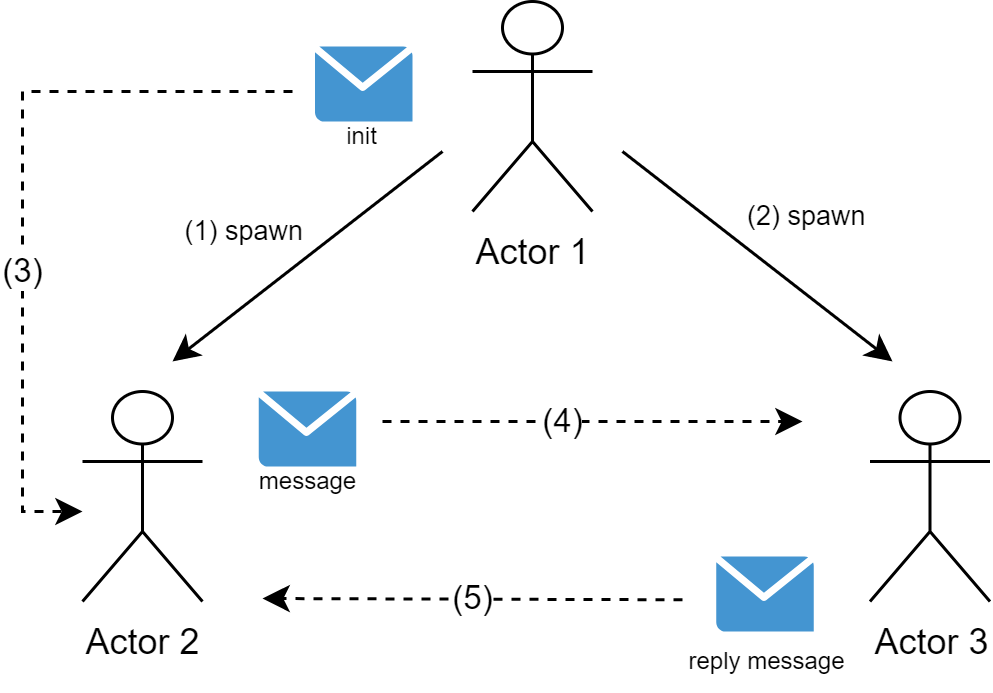
\includegraphics[width=230px]{resources/actors.png}
        \caption{Spawning Actors and Sending Messages}
    \end{centering}
\end{figure}

\subsection{Networking}
Concurrency implies that actors are potentially parallelisable, where multiple actors can process their next message in parallel and thus having the potential to speed up the overall computation. The API must provide an intuitive way to establish a connection with other processes or devices as well to communicate with remote actors. A WebSocket server is used to enable nodes to communicate with each other on a distributed network. The WebSocket server will assign a unique identifier to each connected client which will be broadcasted when the server has the expected number of connected clients. This will allow developers to specify a particular node when utilising the framework.

\begin{figure}[H]
    \begin{centering}
        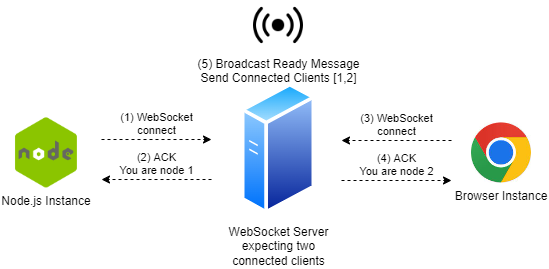
\includegraphics[width=230px]{resources/websocketconnection.png}
        \caption{WebSocket Server Connecting Node.js Instance to a Browser}
    \end{centering}
\end{figure}

Connecting to the server should take the form of an API function call which returns a promise resolving when the server broadcasts to the client that it is ready to forward information to the other connected clients. When the promise is resolved, the developer must be able to refer to actors which exist in remote nodes. API functionality to remotely spawn actors on other nodes would address this requirement as it would allow for one instance to get references to actors it remotely spawned.

The WebSocket server provides distribution for any Node.js or browser client wishing to communicate with actors hosted on other connected clients. However, a developer might want to host multiple instances on a local device to make up for JavaScript's single-threaded nature when distributing actors. The WebSocket server involves an intermediary network hop as well as the network layer, both of which can be avoided by using Node.js~\cite{nodejs} cluster and browser Web Workers~\cite{webworkers}. These methods rely on inter-process communication (IPC) with no network layer and taking advantage of shared memory, while also allowing direct communication between the spawner and the workers. Each of the spawned workers can also be treated as separate instances when connected to the WebSocket server for communication with remote devices.

\begin{figure}[H]
    \begin{centering}
        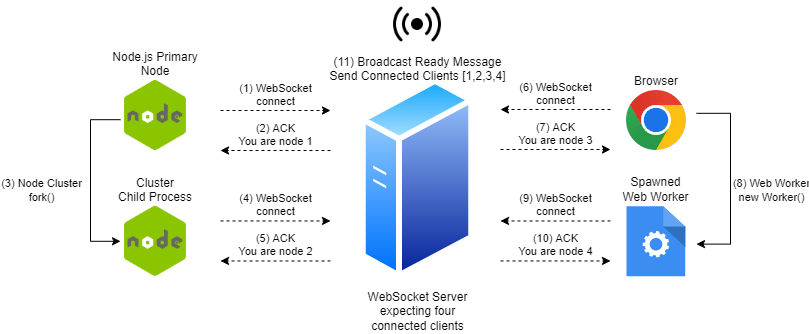
\includegraphics[width=251px]{resources/websocketconnectioncomplex.png}
        \caption{WebSocket Server Connecting Different Types of Processes}
    \end{centering}
\end{figure}

\subsection{API Definition}
The full API definition is as follows. The second function conveniently closes the WebSocket connection and terminates the instance.
\begin{lstlisting}
init = (url: string, timeout: number, numWorkers: number): Promise<object>
closeConnection = ()    //Function to close network connection
spawn = (state: object, behaviour: ActorBehaviour | string): ActorReference
spawnRemote = (node: number, state: object, behaviour: ActorBehaviour, timeout: number): Promise<ActorReference>
send = (actor: ActorReference, message: object): void
terminate = (actor: ActorReference, force: boolean = false)
\end{lstlisting}
\section{Implementation}
\subsection{Anatomy of an Actor}
The internal composition of an actor inside the framework is at the heart of the API's features. An actor takes the form of an object which contains its maintained state as well as its behaviour as an executable function. Each actor stores a name so that it can be uniquely identified in the local instance. The network number assigned by the WebSocket server as well as whether the actor is accepting messages is also stored. The TypeScript interface below defines what an actor is composed of.
\begin{lstlisting}
//TypeScript object interface for an Actor
interface Actor {
    name: string,                       //generated using uuidv4
    node: number,                       //found in global variable
    state: { [key: string]: any },      //given by developer
    behaviour: ActorCallback,           //given by developer
    active: boolean                     //starts with true
}
\end{lstlisting}
When spawning an actor, the state and behaviour are defined by the developer. The name is automatically generated using a uuidv4 package~\cite{uuidv4}. All actors start off as active to indicate that they accept messages. When returning the actor reference to the developer, an issue arises if the whole actor object is returned. Not only does it contain redundant information such as returning the state and behaviour that were just defined by the developer, it also undermines the concept of actor isolation. Since objects are passed by reference in JavaScript, the developer or other actors would be able to modify the actor's state and behaviour through its reference. To protect these attributes, only a subset of the actor object is returned, composed of its name and network number.
\subsection{Communicating with an Actor}
Using the returned ActorReference object from the \textbf{spawn} function, an actor can be uniquely identified across the web. The developer can put in the actor reference inside the \textbf{send} function to send that actor a message. Internally, the framework looks at the actor reference's node number. If it matches the client's network number it resides in, then it will queue the local actor's behaviour on the runtime's event queue. If the actor resides in a remote node, it creates a payload to send over the network. 

When the \textbf{init} function is called, the developer can choose to spawn a number of child processes or web workers. Each of the spawned workers will send to the spawner (primary node) the network number assigned to them by the WebSocket network. The primary node will then send each of the spawned workers of their neighbouring spawned processes' network numbers. This is so that spawned processes can communicate with each other by sending messages to the primary node, which will forward the message to the destination worker using the cluster or web worker API instead of the WebSocket network to avoid the network stack. If the actor resides on a separate device or group of spawned processes, it resorts to using the WebSocket network.
\subsection{Remote Spawning Mechanism}
The \textbf{spawnRemote} function sends a request to spawn an actor to the remote node. The request has embedded within it the string representation of its behaviour which is reconstructed as a function on the recipient end. Similar to the \textbf{send} function, it chooses the fastest transport mechanism to send the spawn request. The primary node is internally aware of the network numbers of the worker nodes it spawned, so it will make use of Cluster IPC to send these requests rather than the slower established WebSocket link through the network.

On the recipient side, the node will spawn an actor with the sent behaviour and initial state. It locally generates the spawned actor's name and embeds it in an acknowledgement sent to the remote spawner. Once this acknowledgement is received by the spawner, it constructs the actor reference using the received actor name and resolves the promise.
\subsection{Actor Runtime}
The JavaScript event loop is responsible for executing the application code. The language's runtime has a queue of messages where each message is mapped to a function which processes that message. The event loop waits for the arrival of a message and processes the queue of messages when there is a backlog in the event queue. Each message is processed to completion before other messages are processed. The Actor Model also maps messages onto functions which act as message handlers. Therefore, the framework's implementation takes advantage of the similar philosophies between the JavaScript runtime and the Actor Model.

The implementation acts as a wrapper of the JavaScript event loop. Once a message is received by an actor, it will schedule the processing of the message on the JavaScript event loop. This is done by scheduling a microtask~\cite{microtasks} which is an event queued to execute before the start of the next event loop~\cite{eventloopbrowser}\cite{eventloopnode}. The microtask is scheduled by creating a promise which is immediately resolved. This behaviour is similar to using Node.js' \textbf{process.nextTick()}~\cite{nexttick} which is more efficient than using the JavaScript's \textbf{setTimeout()} function as it would otherwise schedule a macrotask which executes in the following iteration of the event loop.
\begin{lstlisting}
//Code which schedules the processing of a received message
Promise.resolve().then(() => {
    if (message !== undefined && localActor.active)
        localActor.behaviour(localActor.state, message, { name: localActor.name, node: localActor.node });
})
\end{lstlisting}

Since JavaScript only has one microtask event queue, the order in which messages are sent matches the order in which they are processed by the set of receiving actors. Since JavaScript processes microtasks to completion before processing the next, the implementation ensures that at most one actor is processing a message at any point in time in a single Node.js or browser instance.
\section{Evaluation}
The following hardware and software is used to run benchmarks which quantitaively analyses the framework's performance.
\begin{itemize}
    \item OS --- Ubuntu 20.04 focal (64 bit)
    \item CPU --- Intel Core i7--1065G7. 4 cores up to 3.9GHz with hyper-threading disabled
    \item RAM --- LPDDR4 16GB (2$\times$8GB) at 4267MHz
    \item Node.js – v16.14.0
    \item Google Chrome v100.0.4896.88 (Official Build)
\end{itemize}

\subsection{Micro-Benchmark Performance}
The Savina~\cite{savina} benchmark suite define micro-benchmarks which test specific actor runtime features. The diagram below compares the execution times between the browser and Node.js implementations of Savina's micro-benchmarks. The diagram is followed by an explanation and analysis of each of the executed benchmarks from left to right.
\begin{figure}[H]
    \begin{centering}
        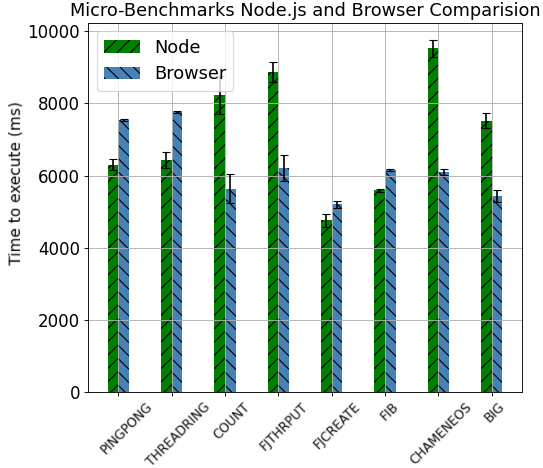
\includegraphics[width=230px]{resources/micro.png}
        \caption{Node.js and Browser Comparison for Micro-Benchmarks}
    \end{centering}
\end{figure}
In general the Node.js and browser implementations for the actor framework have consistent and similar results. Node.js performs worse when a large number of messages are on the event queue.


\subsection{Shared Memory Performance}
The Savina benchmark suite includes parallel benchmarks where multiple actors perform computation in parallel to complete a task. Each of the explored parallel benchmarks benefit from master-worker parallelism, where a master actor farms tasks to worker actors which will start execution in parallel. The workers then report their results to the master which will aggregate the collected data, producing the final result. The framework is tested by first executing the benchmark using only one master and one worker in separate runtimes, where the worker is limited by JavaScript's single-threaded nature.  Next, two workers are spawned on separate runtimes, each of which ideally assigned half of the computational load by the master. Since the framework is tested on a system which houses four cores, the benchmarks are scaled up to four worker runtimes running in parallel. The amount of speedup introduced over running on one worker is tested and plotted below.
\begin{figure}[H]
    \begin{centering}
        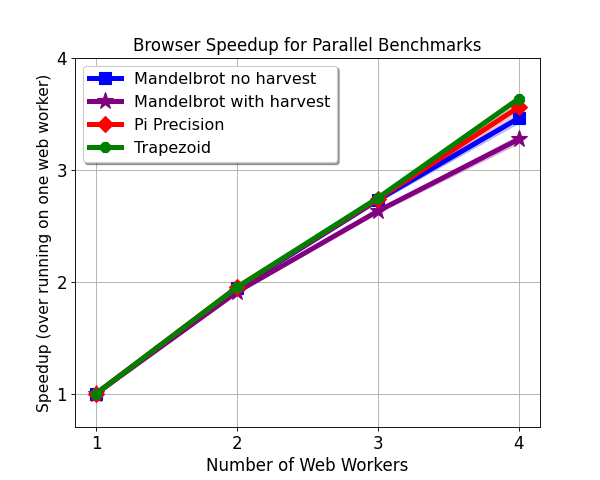
\includegraphics[width=230px]{resources/browser_speedup.png}
        \caption{Browser Shared Memory Speedup}
    \end{centering}
\end{figure}
\subsection{Distributed Memory Performance}
The following benchmark experiments with having actors hosted on a distributed memory. A Raspberry Pi 4 is used to host a WebSocket server which will handle the forwarding of messages between remote devices. The scaling of the Mandelbrot benchmark without harvesting pixel data over Node.js and browsers has already been explored up to four worker instances over shared memory. The diagram below shows the speedup introduced when connecting a new device on the network with the following specifications.
\begin{itemize}
    \item OS --- Windows 10 Home (64 bit)
    \item CPU --- Intel Core i5--10500 6 cores up to 3.10GHz with hyper-threading enabled
    \item RAM --- DDR4 32GB (4$\times$8GB) at 2666MHz
\end{itemize}
In addition to the four workers and master hosted on the four-core device, new workers are incrementally added and connected to the WebSocket server on the new device. While avoiding data harvesting to minimise the network dependency, one can observe a consistent speedup when adding more workers on the second device, with node achieving slightly better speedup with a larger number of workers. Despite network overhead being introduced when distributing actors over the network, the second device makes up for this with its faster processing time.
\begin{figure}[H]
    \begin{centering}
        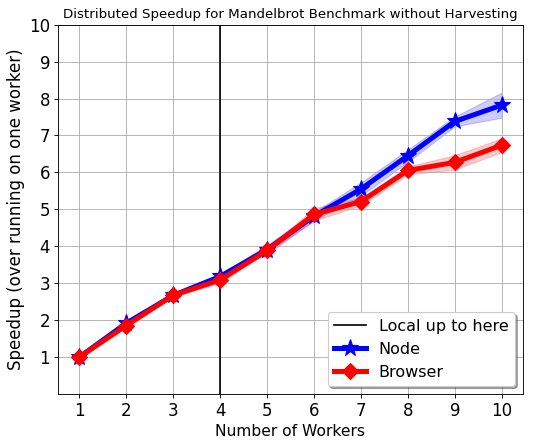
\includegraphics[width=200px]{resources/distributed_memory_speedup.png}
        \caption{Node.js and Browser Comparison for Distributed Memory Speedup}
    \end{centering}
\end{figure}
\section{Conclusions}
Each of the dissertation's four objectives have been fully completed. The two frameworks allow developers to spawn and send messages to actors on local Node.js and browser instances respectively. Messages are processed through the execution of the predefined behaviour of actors (objective 1). Using several web technologies, developers are not limited to a single instance when spawning actors, as they can remotely spawn actors on remote browsers and Node.js instances (objective 2). Once actors are spawned either locally or remotely, the framework internally handles local and remote communication without additional input required by the user (objective 3, location transparency). Finally, the framework is tested through both qualitative and quantitative benchmarks (objective 4).

Each of the dissertation's four objectives have been fully completed. The two frameworks allow developers to spawn and send messages to actors on local Node.js and browser instances respectively. Messages are processed through the execution of the predefined behaviour of actors (objective 1). Using several web technologies, developers are not limited to a single instance when spawning actors, as they can remotely spawn actors on remote browsers and Node.js instances (objective 2). Once actors are spawned either locally or remotely, the framework internally handles local and remote communication without additional input required by the user (objective 3, location transparency).

The developed actor framework is not without its limitations. Distributed clients must connect to a provided WebSocket server to communicate with their peers. Each client must wait for the expected number of clients to connect before being allowed to communicate with each other, and communication over the server introduces an intermediary network hop. The distribution of actors could be done using peer-to-peer WebSocket connections at the cost of more complex synchronisation and requiring each client to listen for connections.
\bibliographystyle{ieeetr}
\bibliography{references}
\end{document}


